\chapter{Chosen Structure Method}
%\section{Chosen Structure Method}

In this section the Waterfall and Iterative method will be described which both are used to structure a project. The concepts of the methods and their strengths and weaknesses will be discussed. This information will be used to support the choice of method. The chosen method and its application in the documentation will be described afterwards.

The waterfall method iterates the project process one time and avoids revision the parts that have already been finished. That means that a part is worked on until it satisfies certain requirements, and then the project members move on to the next part. The iterative method focuses on multiple iterations of the project process and therefore iterating through the project multiple times, expanding the product and documentation each time.

Both methods have their strengths and weaknesses and one method might have a strength that is a weakness for the second method. One of the strengths of the Waterfall method is the consecutive order of progress the structure gives. This gives the project members an overview of how far they are in a specific part or in the overall progress of the project. This overview is obtained as the participants of the project can documentation when a part of the project is finished. Another strength of this method is the ease of setting deadlines for the parts in the documentation and using these deadlines to measure the progress of the project. The consecutive nature of the method can also become a weakness. During the project information can change and this can result in previous parts of the documentation not including or reflecting the new information. This also leads to another weakness which is the question, is the product of the project really complete when the project is done? The project can expand and new information can change, add or subtract requirements for the final product. So it is difficult to conclude that the product is complete when the project is done. 

The iterative method has the strength that it is dynamic. Each iteration of the project process allows the addition of new information and changes. This means that this method adapts very well to new information and changes. When using this method it can be difficult to keep an overview because each iteration adds more information. Each iteration also gives a better understanding of the project context, development and requirements of these. This could lead to an endless circle of improving and expanding the project. So when is the project actually done when using the iterative method? This could prove to be difficult to answer, whereas the Waterfall method gives a structure that restricts the multiple iterations and sets a end point. 

The Waterfall model gives a good structure with an easy overview of progress. It is also a good choice because the system requirements and the goals that have been set, can be defined after each part of the documentation. This allows for confirmation on the goals and requirements that have been set. The Waterfall method will therefore be used in this project.       

When documenting a project using the waterfall method as a structure, it is necessary to write five different parts which covers the project process from start to finish.

\textbf{The analysis part} focuses on getting to know the project in context e.g. to the audience or the environment. This is the part of the documentation that is called problem analysis. It is based on relevant sources e.g. articles, documentations, questionnaires or interviews which satisfies a certain standard of source criticism and relevance. In this project the information is gathered through external sources and interviews. The information is then used to define specific goals and requirements for the following parts of the documentation.

\textbf{The design part} is used to identify design specifications that is needed in a certain product. In our documentation, the design part focused on the principles learned in the courses "Design and Evaluation of User Interfaces" and "Object Oriented Analysis and Design". In this part of the documentation the interface design is modeled by using scenario- based design. The architectural design is created by using Object Oriented Analysis and Design techniques. 

\textbf{The implementation part} is the part in which the software is created. The design specifications is used to make the design, and the needed functionality requirements which was identified through the analysis part is implemented. The outcome of this process in the project is a functional program.

\textbf{The system test} in this part the system is tested to validate if it satisfies the stated requirements and goals in regards to both usability and quality. In the documentation the system is tested to secure that it is of high quality and the usability of the program is also tested. The outcome of this process is a test part included in the report

\textbf{The system in operation} is concerned with describing the system when and after it is published. The documentation incorporates a reflection part and evaluation of what is written previously as a closure of the report.

\begin{figure}[H]
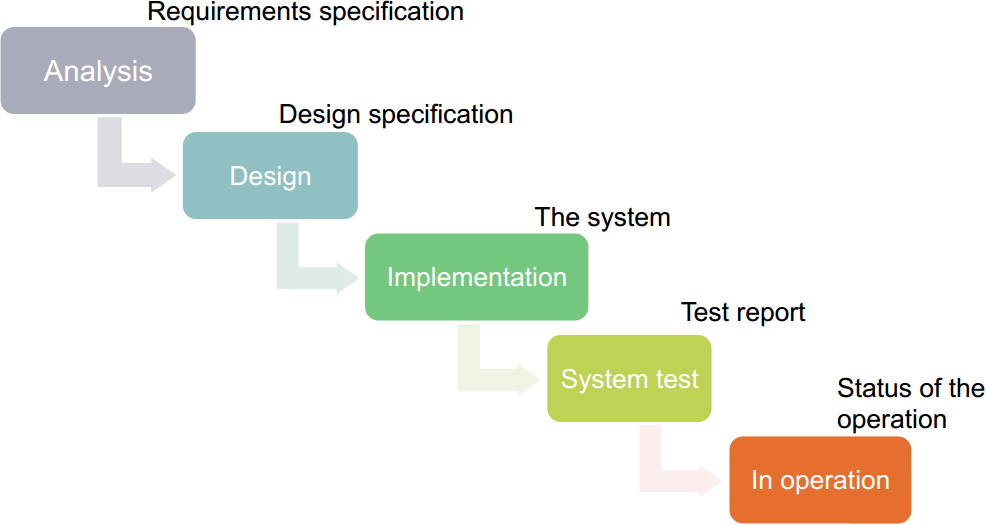
\includegraphics[width=\linewidth, clip=true]{Grafik/FoodPlanner/Waterfall}
\centering
\caption{The waterfall model}
\end{figure}